\documentclass[11pt,onside,a4paper,fleqn]{report}            
\usepackage{graphicx}
\usepackage{subfigure}
\usepackage{epstopdf}
\usepackage{placeins}
\usepackage{amsmath}
\usepackage{array}
\usepackage{bm}
\makeatletter
\renewcommand\arraystretch{2.5}
\renewcommand\normalsize{%
\@setfontsize\normalsize\@xpt\@xiipt
   \abovedisplayskip 4\p@ \@plus2\p@ \@minus8\p@
   \abovedisplayshortskip \z@ \@plus6\p@
   \belowdisplayshortskip 4\p@ \@plus3\p@ \@minus3\p@
   \belowdisplayskip \abovedisplayskip
   \let\@listi\@listI}
\makeatother
 
 
\parindent0pt  \parskip10pt             % make block paragraphs
                           % do not right-justify
\title{\bf Experimental Results}  % Supply information
\author{ \\ LiYuelin\\*\\}
              %   for the title page.
\date{\today}                           %   Use current date.
 
\begin{document}                        % End of preamble, start of text.
\maketitle                              % Print title page.
\pagenumbering{roman}                   % roman page number for toc
\setcounter{page}{1}                    % make it start with "1"
\pagenumbering{arabic}% Start text with arabic 1
 
\chapter{Simulation study}
\hspace{0.8cm}We simulate data from 
\begin{equation}
    \begin{aligned}
        P(Y = 1|x) = \frac{exp(\beta^{T}x + \mu)}{1 + exp(\beta^{T}x + \mu)} 
        \\P(Y = 0|x) = \frac{exp(\beta^{T}x + \mu)}{1 + exp(\beta^{T}x + \mu)}
    \end{aligned} 
\end{equation}
,where the predictors $\bm{x_{i}} = (x_{i1}, x_{i2}, x_{i3}, x_{i4}, x_{i5})^{T}$ are simulated from multivariate
normal distribution with mean 0 and diagonal variance matrix with elements 1 and $\mu_{i}$ are generated from distribution 
$P(\mu_{i} = \alpha) = P(\mu_{i} = -\alpha) = 0.5$.The coefficient vector was set to be 
$\beta = (-0.3, 1, -1, 2, 0.5)^{T}$. We compare the performance of our our estimators using the two concave penalty
functions, namely SCAD and MCP.

\hspace{0.8cm}Next, we investigate the performance of parameter estimation
of the ADMM algorithm with $\tau$ selected via the modified BIC criterion in (5.1) 
with c = 1, 2, 5, 10, 20, 50, 100, 150, 200, 250, 300, 350, 400, 450, 500. 
Tables reports the Monte Carlo mean, median and standard error (s.e.) of the estimated groups
$\hat{K}$ by the SCAD and MCP based on 100 simulation replications. In
addition, to study the estimation accuracy, Table 5.2 reports the
mean and s.e. of the root mean squared errors (RMSE) $\| \hat{\mu}-\mu\| /\sqrt{n}$
and $\| \hat{\beta}-\beta\| /\sqrt{n}$ for the estimated values of $\mu$ and $\beta$, respectively.
The Jaccard coefficient is defined as $\frac{n_{11}}{n_{10}+n_{01}+n_{11}}$, 
where $n_{11}$ is the number of pairs that are comembers in both set A and set B; $n_{10}$ is the number of pairs that are comembers
in set A but not set B, and $n_{01}$ is defined similarly. 

\hspace{0.8cm}The solution paths of the sublogistic model based on a particular sample with $\alpha$ = 0.8 are
shown in Fig. 1.1. It can be seen that for a wide range of tuning parameter $\tau \in (0, 0.65)$, two subgroups are correctly identified by
fitting the model. Tables 1.1 presents the mean,median and standard error for $\hat{K}$ in 20 replications for the model. 
Tables 1.2 presents the mean and standard error of the RMSE for the estimated values of $\mu$ and $\beta$ for the sublogistic model with MCP penalties. The resulting
Jaccard coefficients are summarized in Table 1.3.
\begin{figure}[htbp]
      \centering
      \subfigure[MCP, n = 200, $\alpha = 0.8$]{
      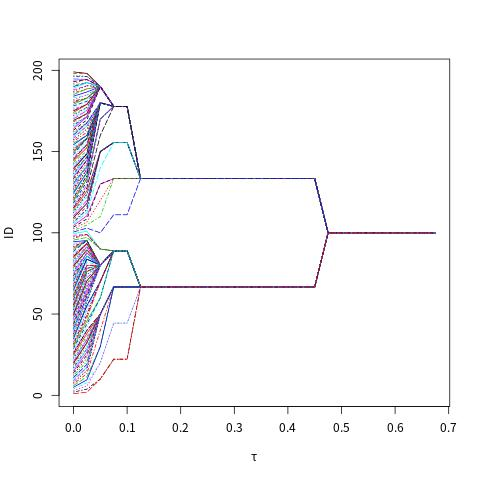
\includegraphics[scale=0.25]{figures/MCP_200_mu=0.8.jpg} \label{1}
      }
      \quad
      \subfigure[MCP, n = 500, $\alpha = 0.8$]{
      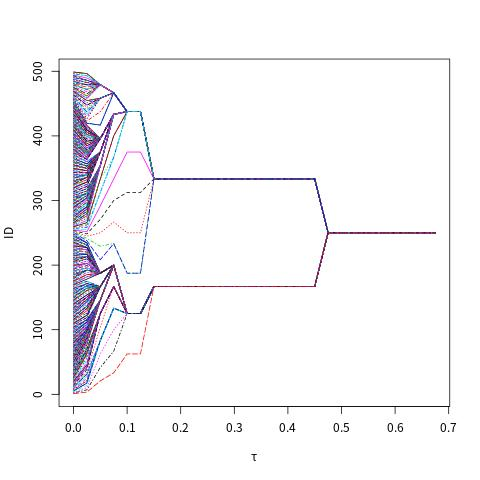
\includegraphics[scale=0.25]{figures/MCP_500_mu=0.8.jpg} \label{2} 
      }
      \quad
      \subfigure[SCAD, n = 200, $\alpha = 0.8$]{
      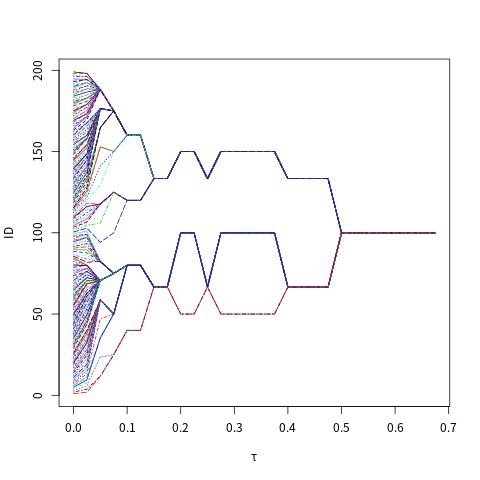
\includegraphics[scale=0.25]{figures/SCAD_200_mu=0.8.jpg}\label{3}
      }
      \quad
      \subfigure[SCAD, n = 500, $\alpha = 0.8$]{
      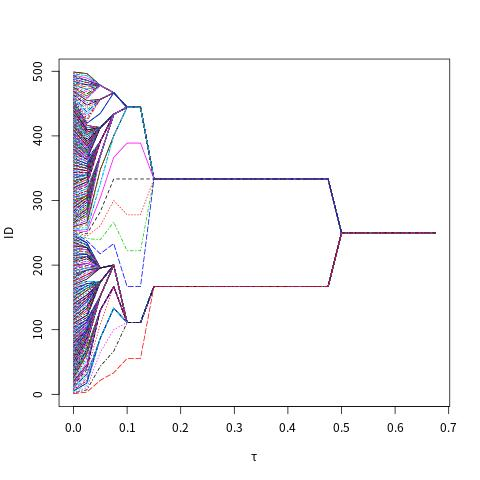
\includegraphics[scale=0.25]{figures/SCAD_500_mu=0.8.jpg}\label{4}
      }
      \caption{\small{Shown are solution paths for the data cluster against $\tau$ by using SCAD and MCP penalties in Example 2.}}
      \end{figure}
      
      
\begin{table}[!h]
    \begin{center}
    \caption{\small{\it{The mean, median and standard error (s.e.) of $\hat{K}$ by the SCAD methods in Example 2.}}}

    \resizebox{\textwidth}{!}{
    \begin{tabular}{|c | c | c c c | c c c | c c c|c c c|c c c|}
    \hline
    \(c\) & $n$    & \multicolumn{3}{|c|}{$\mu=0.8$ }  & \multicolumn{3}{|c|}{$\mu=1$ }   & \multicolumn{3}{|c|}{$\mu=1.2$ } & \multicolumn{3}{|c|}{$\mu=1.4$ }  & \multicolumn{3}{|c|}{$\mu=1.5$ } \\ \hline
          &             &  mean  & median & s.e.   &  mean  & median & s.e.    &  mean & median & s.e.   &  mean  & median & s.e.    &  mean & median & s.e. \\ \hline
    1     & 200       &  4.30	&4.00	&2.60	&4.40   &4.00	 &2.70	 &4.20	 &3.50	 &2.50	 &4.40	 &2.50	 &4.10	 &4.80	 &4.50	 &3.20\\
          & 500       &  5.00	&2.00	&5.50	&4.40	&2.50	&3.40	&6.40	&6.00	&4.90	&5.30	&3.50	&4.10	&6.00	&3.00	&8.10\\ \hline
    2     & 200       &  3.50	&2.00	&2.30	&3.60	&2.50	&2.10	&3.40	&2.50	&1.80	&3.40	&2.50	&1.90	&4.50	&4.00	&3.20\\
          & 500       &  4.00	&2.00	&3.00	&3.80	&2.00	&3.20	&6.20	&4.50	&5.00	&5.00	&3.00	&4.10	&5.80	&3.00	&8.00\\ \hline
    5     & 200       &  2.00	&2.00	&0.00	&2.30	&2.00	&0.80	&2.40	&2.00	&1.00	&2.40	&2.00	&0.81	&2.60	&2.00	&0.94\\
          & 500       &  2.60	&2.00	&1.80	&3.20	&2.00	&3.00	&3.60	&2.00	&3.80	&4.10	&2.00	&4.10	&3.80	&2.00	&3.20\\ \hline
    10    & 200       &  2.00	&2.00	&0.00	&2.00	&2.00	&0.22	&2.00	&2.00	&0.00	&2.20	&2.00	&0.52	&2.20	&2.00	&0.62\\
          & 500       &  2.00	&2.00	&0.22	&2.20	&2.00	&0.79	&3.00	&2.00	&3.40	&3.40	&2.00	&2.60	&2.60	&2.00	&1.60\\ \hline
    20    & 200       &  1.90	&2.00	&0.31	&2.00	&2.00	&0.22	&2.00	&2.00	&0.00	&2.00	&2.00	&0.00	&2.10	&2.00	&0.45\\
          & 500       &  2.00	&2.00	&0.22	&2.20	&2.00	&0.49	&2.00	&2.00	&0.00	&2.30	&2.00	&0.57	&2.20	&2.00	&0.64\\ \hline
    50    & 200       &  1.90	&2.00	&0.31	&2.00	&2.00	&0.22	&2.00	&2.00	&0.00	&2.00	&2.00	&0.00	&2.10	&2.00	&0.45\\
          & 500       &  2.00	&2.00	&0.22	&2.20	&2.00	&0.49	&2.00	&2.00	&0.00	&2.30	&2.00	&0.57	&2.20	&2.00	&0.64\\ \hline
    100   & 200       &  1.70	&2.00	&0.47	&2.00	&2.00	&0.32	&2.00	&2.00	&0.00	&2.00	&2.00	&0.00	&2.10	&2.00	&0.45\\
          & 500       &  2.00	&2.00	&0.22	&2.20	&2.00	&0.49	&2.00	&2.00	&0.00	&2.30	&2.00	&0.57	&2.20	&2.00	&0.64\\ \hline
    200   & 200       &  1.40	&1.00	&0.49	&1.60	&2.00	&0.49	&2.00	&2.00	&0.00	&2.00	&2.00	&0.00	&2.10	&2.00	&0.45\\
          & 500       &  2.00	&2.00	&0.22	&2.20	&2.00	&0.49	&2.00	&2.00	&0.00	&2.30	&2.00	&0.57	&2.20	&2.00	&0.64\\ \hline
    250   & 200       &  1.20	&1.00	&0.37	&1.60	&2.00	&0.51	&2.00	&2.00	&0.22	&2.00	&2.00	&0.00	&2.10	&2.00	&0.45\\
          & 500       &  2.00	&2.00	&0.22	&2.20	&2.00	&0.49	&2.00	&2.00	&0.00	&2.30	&2.00	&0.57	&2.20	&2.00	&0.64\\ \hline
    300   & 200       &  1.00	&1.00	&0.00	&1.40	&1.00	&0.50	&1.80	&2.00	&0.37	&2.00	&2.00	&0.00	&2.10	&2.00	&0.45\\
          & 500       &  2.00	&2.00	&0.22	&2.20	&2.00	&0.49	&2.00	&2.00	&0.00	&2.30	&2.00	&0.57	&2.20	&2.00	&0.64\\ \hline
    350   & 200       &  1.00	&1.00	&0.00	&1.20	&1.00	&0.41	&1.80	&2.00	&0.44	&2.00	&2.00	&0.00	&2.10	&2.00	&0.45\\
          & 500       &  2.00	&2.00	&0.22	&2.20	&2.00	&0.49	&2.00	&2.00	&0.00	&2.30	&2.00	&0.57	&2.20	&2.00	&0.64\\ \hline
    400   & 200       &  1.00	&1.00	&0.00	&1.00	&1.00	&0.22	&1.40	&1.00	&0.51	&2.00	&2.00	&0.00	&2.10	&2.00	&0.45\\
          & 500       &  2.00	&2.00	&0.32	&2.20	&2.00	&0.49	&2.00	&2.00	&0.00	&2.30	&2.00	&0.57	&2.20	&2.00	&0.64\\ \hline
    450   & 200       &  1.00	&1.00	&0.00	&1.00	&1.00	&0.22	&1.40	&1.00	&0.50	&2.00	&2.00	&0.00	&2.10	&2.00	&0.45\\
          & 500       &  1.80	&2.00	&0.37	&2.20	&2.00	&0.49	&2.00	&2.00	&0.00	&2.30	&2.00	&0.57	&2.20	&2.00	&0.64\\ \hline
    500   & 200       &  1.00	&1.00	&0.00	&1.00	&1.00	&0.00	&1.40	&1.00	&0.49	&2.00	&2.00	&0.00	&2.10	&2.00	&0.45\\
          & 500       &  1.80	&2.00	&0.37	&2.00	&2.00	&0.32	&2.00	&2.00	&0.00	&2.30	&2.00	&0.57	&2.20	&2.00	&0.64\\ \hline
    \end{tabular}}
    \end{center}
    \end{table}

\begin{table}[!h]
    \begin{center}
    \caption{\small{\it{The mean and standard error (s.e.) (shown in parentheses) of the RMSE for the estimated
    values of $\mu$ and $\beta$ for the MCP methods.}}}
    \label{table.mubeta1}
    \resizebox{\textwidth}{!}{
    \begin{tabular}{|c | c | c c c c c| c c c c c| }
    \hline
        &            & \multicolumn{5}{|c|}{$\mu$}  &  \multicolumn{5}{|c|}{$\beta$} \\ \hline
    \(c\) & \(n\) &  $\mu=0.8$  & $\mu=1$   & $\mu=1.2$  & $\mu=1.4$ & $\mu=1.5$ &  $\mu=0.8$  & $\mu=1$   & $\mu=1.2$  & $\mu=1.4$ & $\mu=1.5$ \\ \hline
    1       & 200      &  $0.2255_{(0.1283)}$   & $0.2702_{(0.1015)}$   &  $0.2628_{(0.1587)}$  &  $0.2495_{(0.1432)}$  & $0.2722_{(0.1221)}$   &  $0.2255_{(0.1283)}$  & $0.2702_{(0.1015)}$     &  $0.2628_{(0.1587)}$   &  $0.2495_{(0.1432)}$     & $0.2722_{(0.1221)}$ \\
            & 500      &  $0.1255_{(0.1052)}$   & $0.1350_{(0.1024)}$   &  $0.1470_{(0.0917)}$  &  $0.1413_{(0.1035)}$  & $0.1347_{(0.1100)}$   &  $0.1290_{(0.0420}$  & $0.1315_{(0.0493)}$     &  $0.1280_{(0.0495)}$   &  $0.1388_{(0.0453)}$     & $0.1374_{(0.0328)}$ \\ \hline
    2       & 200      &  $0.2199_{(0.1309)}$   & $0.2647_{(0.1045)}$   &  $0.2549_{(0.1602)}$  &  $0.2459_{(0.1435)}$  & $0.2672_{(0.1247)}$   &  $0.2145_{(0.0766)}$  & $0.2278_{(0.1036)}$     &  $0.1966_{(0.0794)}$   &  $0.2214_{(0.0548)}$     & $0.2234_{(0.0560)}$ \\
            & 500      &  $0.1222_{(0.1044)}$   & $0.1263_{(0.1052)}$   &  $0.1412_{(0.0970)}$  &  $0.1349_{(0.1020)}$  & $0.1304_{(0.1085)}$   &  $0.1287_{(0.0421)}$  & $0.1316_{(0.0493)}$     &  $0.1283_{(0.0491)}$   &  $0.1389_{(0.0454)}$     & $0.1375_{(0.0328)}$ \\ \hline
    5       & 200      &  $0.2015_{(0.1449)}$   & $0.2490_{(0.1155)}$   &  $0.2395_{(0.1635)}$  &  $0.2120_{(0.1649)}$  & $0.2233_{(0.1340)}$   &  $0.2144_{(0.0764)}$  & $0.2249_{(0.1033)}$     &  $0.1949_{(0.0789)}$   &  $0.2190_{(0.0537)}$     & $0.2225_{(0.0561)}$ \\
            & 500      &  $0.1090_{(0.1115)}$   & $0.1202_{(0.1079)}$   &  $0.1068_{(0.0950)}$  &  $0.1183_{(0.1028)}$  & $0.1089_{(0.1002)}$   &  $0.1290_{(0.0420)}$  & $0.1320_{(0.0492)}$     &  $0.1284_{(0.0493)}$   &  $0.1387_{(0.0454)}$     & $0.1371_{(0.0331)}$ \\ \hline
    10      & 200      &  $0.2015_{(0.1449)}$   & $0.2457_{(0.1184)}$   &  $0.2278_{(0.1713)}$  &  $0.2058_{(0.1653)}$  & $0.2137_{(0.1296)}$   &  $0.2144_{(0.0764)}$  & $0.2250_{(0.1035)}$     &  $0.1936_{(0.0797)}$   &  $0.2191_{(0.0537)}$     & $0.2229_{(0.0559)}$ \\
            & 500      &  $0.1076_{(0.1085)}$   & $0.1136_{(0.1031)}$   &  $0.0971_{(0.0906)}$  &  $0.1080_{(0.1008)}$  & $0.0892_{(0.0787)}$   &  $0.1289_{(0.0420)}$  & $0.1317_{(0.0492)}$     &  $0.1283_{(0.0494)}$   &  $0.1387_{(0.0452)}$     & $0.1372_{(0.0330)}$ \\ \hline
    20      & 200      &  $0.2559_{(0.2560)}$   & $0.2457_{(0.1184)}$   &  $0.2278_{(0.1713)}$  &  $0.1978_{(0.1650)}$  & $0.2098_{(0.1287)}$   &  $0.2130_{(0.0733)}$  & $0.2250_{(0.1035)}$     &  $0.1936_{(0.0797)}$   &  $0.2184_{(0.0550)}$     & $0.2220_{(0.0552)}$ \\
            & 500      &  $0.1076_{(0.1085)}$   & $0.1130_{(0.1021)}$   &  $0.0913_{(0.0748)}$  &  $0.0916_{(0.0770)}$  & $0.0852_{(0.0701)}$   &  $0.1289_{(0.0420)}$  & $0.1317_{(0.0492)}$     &  $0.1278_{(0.0491)}$   &  $0.1390_{(0.0452)}$     & $0.1372_{(0.0330)}$ \\ \hline
    50      & 200      &  $0.2559_{(0.2560)}$   & $0.2457_{(0.1184)}$   &  $0.2278_{(0.1713)}$  &  $0.1978_{(0.1650)}$  & $0.2098_{(0.1287)}$   &  $0.2130_{(0.0733)}$  & $00.2250_{(0.1035)}$     &  $0.1936_{(0.0797)}$   &  $0.2184_{(0.0550)}$     & $0.2220_{(0.0552)}$ \\
            & 500      &  $0.1076_{(0.1085)}$   & $0.1130_{(0.1021)}$   &  $0.0913_{(0.0748)}$  &  $0.0916_{(0.0770)}$  & $0.0852_{(0.0701)}$   &  $0.1289_{(0.0420)}$  & $0.1317_{(0.0492)}$     &  $0.1278_{(0.0491)}$   &  $0.1390_{(0.0452)}$     & $0.1372_{(0.0330)}$ \\ \hline
    100     & 200      &  $0.3951_{(0.3238)}$	&  $0.2848_{(0.2177)}$	&  $0.2278_{(0.1713)}$	&  $0.1978_{(0.1650)}$	&  $0.2098_{(0.1287)}$	&  $0.2147_{(0.0701)}$	&  $0.2251_{(0.1035)}$	&  $0.1936_{(0.0797)}$	    &  $0.2184_{(0.0550)}$	&  $0.2220_{(0.0552)}$ \\
            & 500      &  $0.1076_{(0.1085)}$	&  $0.1130_{(0.1021)}$	&  $0.0913_{(0.0748)}$	&  $0.0916_{(0.0770)}$	&  $0.0852_{(0.0701)}$	&  $0.1289_{(0.0420)}$	&  $0.1317_{(0.0492)}$	&  $0.1278_{(0.0491)}$	&  $0.1390_{(0.0452)}$	&  $0.1372_{(0.0330)}$ \\ \hline
    200     & 200      &  $0.6075_{(0.3318)}$	&  $0.5350_{(0.3818)}$	&  $0.2278_{(0.1713)}$	&  $0.1978_{(0.1650)}$	&  $0.2098_{(0.1287)}$	&  $0.2286_{(0.0663)}$	&  $0.2267_{(0.1043)}$	&  $0.1936_{(0.0797)}$	&  $0.2184_{(0.0550)}$	&  $0.2220_{(0.0552)}$\\
            & 500      &  $0.1076_{(0.1085)}$	&  $0.1130_{(0.1021)}$	&  $0.0913_{(0.0748)}$	&  $0.0916_{(0.0770)}$	&  $0.0852_{(0.0701)}$	&  $0.1289_{(0.0420)}$	&  $0.1317_{(0.0492)}$	&  $0.1278_{(0.0491)}$	&  $0.1390_{(0.0452)}$	&  $0.1372_{(0.0330)}$\\ \hline
    250     & 200      &  $0.7297_{(0.2649)}$	&  $0.6158_{(0.3902)}$	&  $0.2785_{(0.2777)}$	&  $0.1978_{(0.1650)}$	&  $0.2098_{(0.1287)}$	&  $0.2349_{(0.0649)}$	&  $0.2302_{(0.1044)}$	&  $0.2020_{(0.0871)}$	&  $0.2184_{(0.0550)}$	&  $0.2220_{(0.0552)}$\\
            & 500      &  $0.1076_{(0.1085)}$	&  $0.1130_{(0.1021)}$	&  $0.0913_{(0.0748)}$	&  $0.0916_{(0.0770)}$	&  $0.0852_{(0.0701)}$	&  $0.1289_{(0.0420)}$	&  $0.1317_{(0.0492)}$	&  $0.1278_{(0.0491)}$	&  $0.1390_{(0.0452)}$	&  $0.1372_{(0.0330)}$\\ \hline
    300     & 200      &  $0.8325_{(0.0417)}$	&  $0.7195_{(0.3963)}$	&  $0.3892_{(0.3879)}$	&  $0.1978_{(0.1650)}$	&  $0.2098_{(0.1287)}$	&  $0.2393_{(0.0647)}$	&  $0.2286_{(0.1051)}$	&  $0.2060_{(0.0896)}$	&  $0.2184_{(0.0550)}$	&  $0.2220_{(0.0552)}$ \\
            & 500      &  $0.1076_{(0.1085)}$	&  $0.1130_{(0.1021)}$	&  $0.0913_{(0.0748)}$	&  $0.0916_{(0.0770)}$	&  $0.0852_{(0.0701)}$	&  $0.1289_{(0.0420)}$	&  $0.1317_{(0.0492)}$	&  $0.1278_{(0.0491)}$	&  $0.1390_{(0.0452)}$	&  $0.1372_{(0.0330)}$\\ \hline
    350     & 200      &  $0.8325_{(0.0417)}$	&  $0.8675_{(0.3446)}$	&  $0.5019_{(0.4444)}$	&  $0.1978_{(0.1650)}$	&  $0.2098_{(0.1287)}$	&  $0.2393_{(0.0647)}$	&  $0.2339_{(0.0935)}$	&  $0.2164_{(0.0816)}$	&  $0.2184_{(0.0550)}$	&  $0.2220_{(0.0552)}$\\
            & 500      &  $0.1076_{(0.1085)}$	&  $0.1130_{(0.1021)}$	&  $0.0913_{(0.0748)}$	&  $0.0916_{(0.0770)}$	&  $0.0852_{(0.0701)}$	&  $0.1289_{(0.0420)}$	&  $0.1317_{(0.0492)}$	&  $0.1278_{(0.0491)}$	&  $0.1390_{(0.0452)}$	&  $0.1372_{(0.0330)}$\\ \hline
    400     & 200      &  $0.8325_{(0.0417)}$	&  $0.9917_{(0.1813)}$	&  $0.7881_{(0.5028)}$	&  $0.1978_{(0.1650)}$	&  $0.2098_{(0.1287)}$	&  $0.2393_{(0.0647)}$	&  $0.2484_{(0.0877)}$	&  $0.2385_{(0.0795)}$	&  $0.2184_{(0.0550)}$	&  $0.2220_{(0.0552)}$\\
            & 500      &  $0.1457_{(0.1879)}$	&  $.1130_{(0.1021)}$	&  $0.0913_{(0.0748)}$	&  $0.0916_{(0.0770)}$	&  $0.0852_{(0.0701)}$	&  $0.1294_{(0.0423)}$	&  $0.1317_{(0.0492)}$	&  $0.1278_{(0.0491)}$	&  $0.1390_{(0.0452)}$	&  $0.1372_{(0.0330)}$\\  \hline
    450     & 200      &  $0.8325_{(0.0417)}$	&  $0.9917_{(0.1813)}$	&  $0.8444_{(0.4813)}$	&  $0.1978_{(0.1650)}$	&  $0.2098_{(0.1287)}$	&  $0.2393_{(0.0647)}$	&  $0.2484_{(0.0877)}$	&  $0.2436_{(0.0789)}$	&  $0.2184_{(0.0550)}$	&  $0.2220_{(0.0552)}$\\
            & 500      &  $0.2196_{(0.2725)}$	&  $0.1130_{(0.1021)}$	&  $0.0913_{(0.0748)}$	&  $0.0916_{(0.0770)}$	&  $0.0852_{(0.0701)}$	&  $0.1272_{(0.0308)}$	&  $0.1317_{(0.0492)}$	&  $0.1278_{(0.0491)}$	&  $0.1390_{(0.0452)}$	&  $0.1372_{(0.0330)}$\\  \hline
    500     & 200      &  $0.8325_{(0.0417)}$	&  $1.0310_{(0.0255)}$	&  $0.8929_{(0.4699)}$	&  $0.1978_{(0.1650)}$	&  $0.2098_{(0.1287)}$	&  $0.2393_{(0.0647)}$	&  $0.2508_{(0.0922)}$	&  $0.2479_{(0.0799)}$	&  $0.2184_{(0.0550)}$	&  $0.2220_{(0.0552)}$\\
            & 500      &  $0.2196_{(0.2725)}$	&  $0.1603_{(0.2223)}$	&  $0.0913_{(0.0748)}$	&  $0.0916_{(0.0770)}$	&  $0.0852_{(0.0701)}$	&  $0.1272_{(0.0308)}$	&  $0.1395_{(0.0644)}$	&  $0.1278_{(0.0491)}$	&  $0.1390_{(0.0452)}$	&  $0.1372_{(0.0330)}$\\  \hline
    \end{tabular}}
    \end{center}
\end{table}

\renewcommand\arraystretch{1.2} 
\begin{table}[!h]
    \begin{center}
    \caption{\small{\it{Jaccard coefficients}}}
    \label{table.p1}

    \begin{tabular}{|c | c | c | c | c | c | c | }
    \hline
    \(c\)    & \(n\)       & $\mu=0.8$  & $\mu=1$   & $\mu=1.2$ & $\mu=1.4$ & $\mu=1.5$\\ \hline
    1           & 200      &  $0.646$	&  $0.806$	&  $0.708$	&  $0.843$	&  $0.860$\\
                & 500      &  $0.726$	&  $0.645$	&  $0.477$	&  $0.671$	&  $0.606$\\ \hline
    2           & 200      &  $0.682$	&  $0.861$	&  $0.775$	&  $0.867$	&  $0.860$\\
                & 500      &  $0.772$	&  $0.724$	&  $0.510$	&  $0.734$	&  $0.635$\\ \hline
    5           & 200      &  $0.875$	&  $0.975$	&  $0.867$	&  $0.958$	&  $0.967$\\
                & 500      &  $0.960$	&  $0.803$	&  $0.739$	&  $0.807$	&  $0.775$\\ \hline
    10          & 200      &  $0.875$	&  $0.975$	&  $0.875$	&  $0.975$	&  $1.000$\\
                & 500      &  $1.000$	&  $0.915$	&  $0.817$	&  $0.849$	&  $0.928$\\ \hline
    20          & 200      &  $0.850$	&  $0.975$	&  $0.875$	&  $1.000$	&  $1.000$\\
                & 500      &  $1.000$	&  $0.945$	&  $0.875$	&  $0.967$	&  $0.967$\\ \hline
    50          & 200      &  $0.850$	&  $0.975$	&  $0.875$	&  $1.000$	&  $1.000$\\
                & 500      &  $1.000$	&  $0.945$	&  $0.875$	&  $0.967$	&  $0.967$\\ \hline
    100         & 200      &  $0.775$	&  $0.950$	&  $0.875$	&  $1.000$	&  $1.000$\\
                & 500      &  $1.000$	&  $0.945$	&  $0.875$	&  $0.967$	&  $0.967$\\ \hline
    200         & 200      &  $0.600$	&  $0.800$	&  $0.875$	&  $1.000$	&  $1.000$\\
                & 500      &  $1.000$	&  $0.945$	&  $0.875$	&  $0.967$	&  $0.967$\\ \hline
    250         & 200      &  $0.550$	&  $0.750$	&  $0.850$	&  $1.000$	&  $1.000$\\
                & 500      &  $1.000$	&  $0.945$	&  $0.875$	&  $0.967$	&  $0.967$\\ \hline
    300         & 200      &  $0.500$	&  $0.675$	&  $0.800$	&  $1.000$	&  $1.000$\\
                & 500      &  $1.000$	&  $0.945$	&  $0.875$	&  $0.967$	&  $0.967$\\ \hline
    350         & 200      &  $0.500$	&  $0.575$	&  $0.750$	&  $1.000$	&  $1.000$\\
                & 500      &  $1.000$	&  $0.945$	&  $0.875$	&  $0.967$	&  $0.967$\\ \hline
    400         & 200      &  $0.500$	&  $0.525$	&  $0.600$	&  $1.000$	&  $1.000$\\
                & 500      &  $0.975$	&  $0.945$	&  $0.875$	&  $0.967$	&  $0.967$\\ \hline
    450         & 200      &  $0.500$	&  $0.525$	&  $0.575$	&  $1.000$	&  $1.000$\\
                & 500      &  $0.925$	&  $0.945$	&  $0.875$	&  $0.967$	&  $0.967$\\ \hline
    500         & 200      &  $0.500$	&  $0.500$	&  $0.550$	&  $1.000$	&  $1.000$\\
                & 500      &  $0.925$	&  $0.950$	&  $0.875$	&  $0.967$	&  $0.967$\\ \hline
    \end{tabular}
    \end{center}
\end{table}
 
\chapter{Empirical example}

\hspace{0.8cm}Nowadays, telecom industry faces fierce com-petition in satisfying its customers. The role of churn prediction system is not only restricted to accurately predict churners but also to interpret customer churn behavior. 
Experiments are conducted on the Cell2cell churn datasets which 

\hspace{0.8cm}First, missing value imputation is applied. Missing values are treated differently based on the percentage of missing values in
an attribute. 
Imputation procedures are used for attributes with more than 5 of the values missing. 
Depending on the variable, zero imputation, median imputation or modus imputation is used.
Dummy variables are created flagging variables where missing variables are imputed. 
For attributes with less than $5\%$ of the values missing, the instances containing the missing value are removed from the data in order to limit the impact of imputation
procedures. 
Categorical variables are transformed into binary variables using dummy encoding. 
This technique creates $v–1$ dummy variables, where $v$ equals the number of distinct values of the categorical variables. 
These newly created variables indicate the presence or absence of a particular characteristic.

\hspace{0.8cm}Second, outlier detection and treatment is applied. Outliers are
unusual values that are typically defined as being more than three
standard deviations away from a variable’s mean value.

\hspace{0.8cm}A last preprocessing step involves undersampling. Typically, the class variable in a churn prediction setting is heavily skewed, i.e.
the number of churners is often much lower than the number of non-churners.

\hspace{0.8cm}Considering that a classifier trained on a small set of well-chosen and highly predictive variables will have better predictive performance, 
We use fisher score which is simple but effective to reduce e the number of variables. The fisher score is defined as
\begin{equation}
          Fisher \  score = \frac{\|\overline{X}_{c} - \overline{X}_{nc}\|}{\sqrt{S_{c}^{2}+S_{nc}^{2}}} 
\end{equation}  
where $\overline{X}_{c}$ and $\overline{X}_{nc}$ the mean value, and $S_{c}^{2}$ and $S_{nc}^{2}$ the variance of an independent variable for respectively churners and non-churners.
Table 9 gives an overview of the selected variables through applying the fisher selection.
\renewcommand\arraystretch{1.2} 
\begin{table}[!h]

    \caption{\small{\it{Overview of selected variables in cell2cell dataset.}}}
    \label{table.variable}
    \begin{tabular}{c | cccccccc }
    \hline
      Variable          & Definition      \\ \hline
      Callwait          & Mean number of call waiting calls\\
      changem           & $\%$ change in minutes of use\\ 
      creditde          & Low credit rating – de\\
      custcare          & Mean number of customer care calls\\
      directas          & Mean number of director assisted calls\\
      eqpdays           & Number of days of the current equipment\\
      incalls           & Mean number of inbound voice calls\\
      mou               & Mean monthly minutes of use\\
      opeakvce          & Mean number of in and out off-peak voice call\\
      outcalls          & Mean number of outbound voice calls\\
      phones            & $\#$ handsets issued\\
      recchrge          & Mean total recurring charge\\
      retcalls          & Number of calls previously made to the retention team\\
      revenue           & Mean monthly revenue\\
      price             & Handset price\\
      webcap            & Handset is web capable\\ \hline
    \end{tabular}
\end{table}

\hspace{0.8cm}We fit the data with two LLM models that constructs a decision tree in the first step to identify homogenous customer segments 
and in a second step applies classifier to each of these segments. One is the ordinary logistic regressions and the other model is the sublogistic regressions. 
Then, we plot the kernel density estimates of the Pearson residuals of the first model in 残差图. The Pearson residuals are defined as$r_{i} = \frac{Y_{i}-\widehat{E(Y_{i})}}{\sqrt{\widehat{Var(Y_{i})}}}$.
It is clearly seen that after adjusting for the effects of covariates, the distribution of residuals still shows multiple modes.
\begin{figure}[htbp]
      \centering
      \subfigure[Pearson residual of Group1]{
      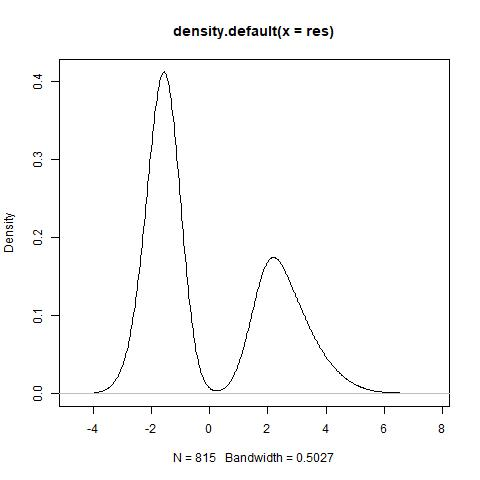
\includegraphics[scale=0.25]{figures/group 1 .jpg} \label{logisGroup1}
      }
      \quad
      \subfigure[Pearson residual of Group2]{
      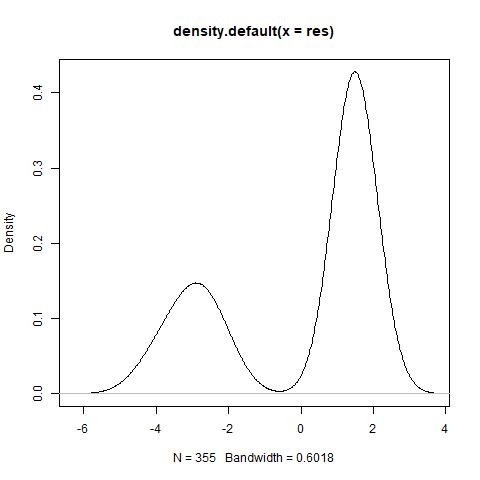
\includegraphics[scale=0.25]{figures/group 2 .jpg} \label{logisGroup2} 
      }
      \quad
      \subfigure[Pearson residual of Group3]{
      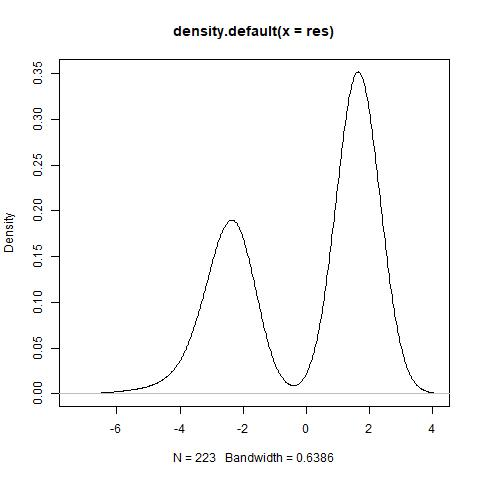
\includegraphics[scale=0.25]{figures/group 3 .jpg}\label{logisGroup3}
      }
      \quad
      \subfigure[Pearson residual of Group4]{
      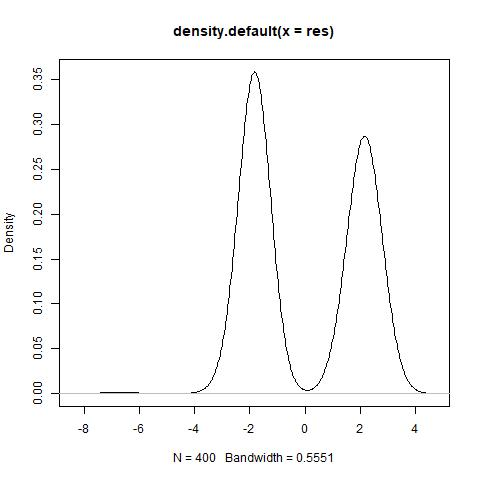
\includegraphics[scale=0.25]{figures/group 4 .jpg}\label{logisGroup4}
      }
      \quad
      \subfigure[Pearson residual of Group5]{
      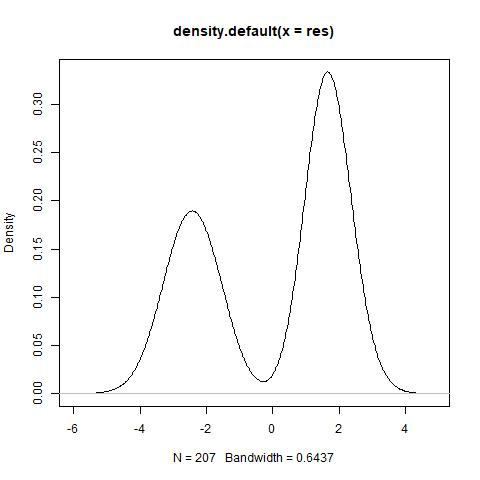
\includegraphics[scale=0.25]{figures/group 5 .jpg}\label{logisGroup5}
      }
      \caption{\small{Kernel density plot of the Pearson residuals of each group identifed by the LLM model with ordinary logistic regressions.}}
      \end{figure}
      
\hspace{0.8cm}Next, we use sublogistic regressions and identify subgroups by our proposed ADMM algorithm and plot the kernel density estimates of the Pearson residuals. As shown in 残差图, 
after incorporating the heterogeneous latent intercepts, the distribution of fitted residuals mostly has a single mode, i.e., the residuals follow a homogeneous distribution.

\begin{figure}[htbp]
      \centering
      \subfigure[Pearson residual of Group1 subgroup1]{
      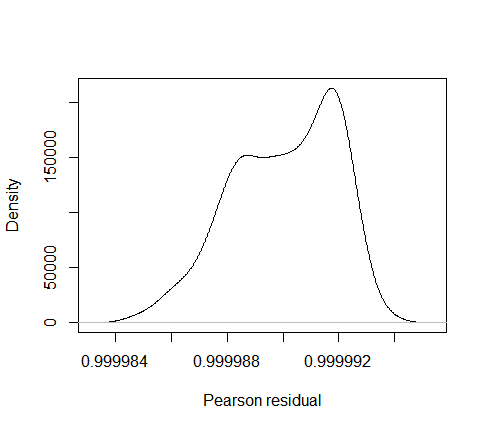
\includegraphics[scale=0.25]{figures/group1_1.png} \label{sublogisGroup1Subgroup1}
      }
      \quad
      \subfigure[Pearson residual of Group1 subgroup2]{
      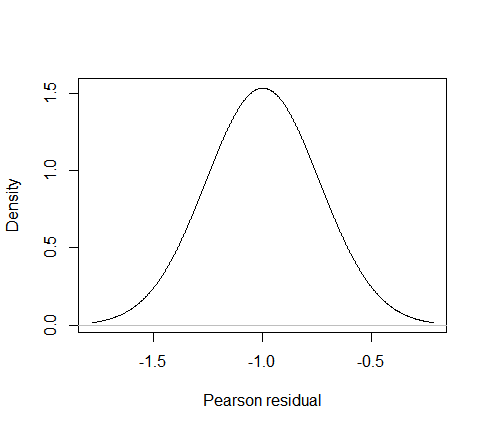
\includegraphics[scale=0.25]{figures/group1_2.png} \label{sublogisGroup1Subgroup2} 
      }
      \caption{\small{Kernel density plot of the Pearson residuals of subgroups in Group1 identifed by the LLM model with sublogistic regressions.}}
      \end{figure}
            
\begin{figure}[htbp]
      \centering
      \subfigure[Pearson residual of Group2 subgroup1]{
      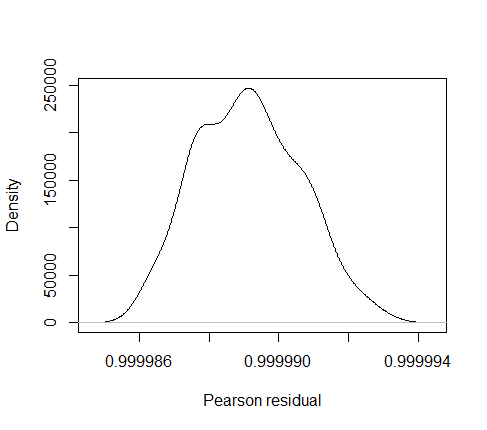
\includegraphics[scale=0.25]{figures/group2_1.png}\label{sublogisGroup2Subgroup1}
      }
      \quad
      \subfigure[Pearson residual of Group2 subgroup2]{
      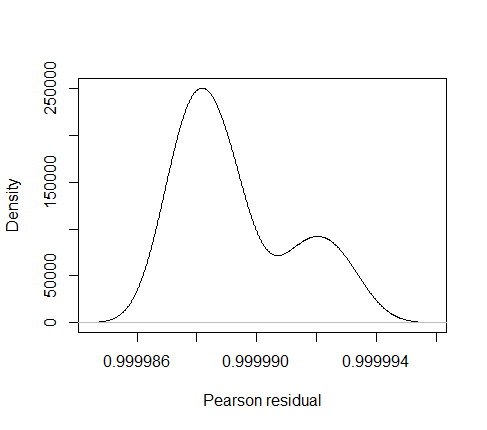
\includegraphics[scale=0.25]{figures/group2_2.png}\label{sublogisGroup2Subgroup2}
      }
      \quad
      \subfigure[Pearson residual of Group2 subgroup3]{
      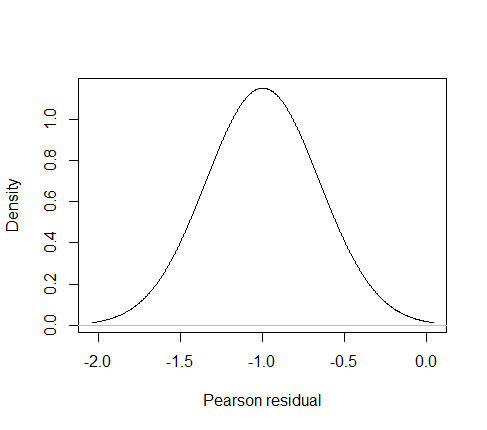
\includegraphics[scale=0.25]{figures/group2_3.png}\label{sublogisGroup2Subgroup3}
      }
      \caption{\small{Kernel density plot of the Pearson residuals of subgroups in Group2 identifed by the LLM model with sublogistic regressions.}}
      \end{figure}

\begin{figure}[htbp]
      \centering
      \subfigure[Pearson residual of Group3 subgroup1]{
      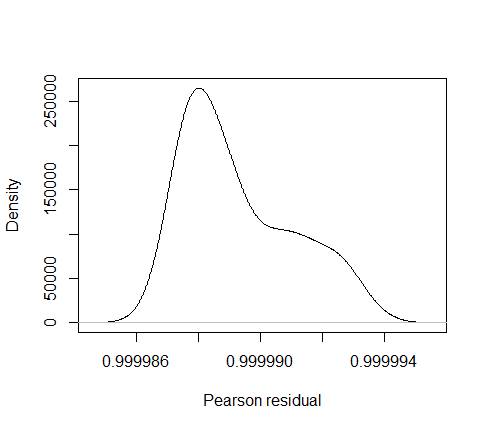
\includegraphics[scale=0.25]{figures/group3_1.png}\label{sublogisGroup3Subgroup1}
      }
      \quad
      \subfigure[Pearson residual of Group3 subgroup2]{
      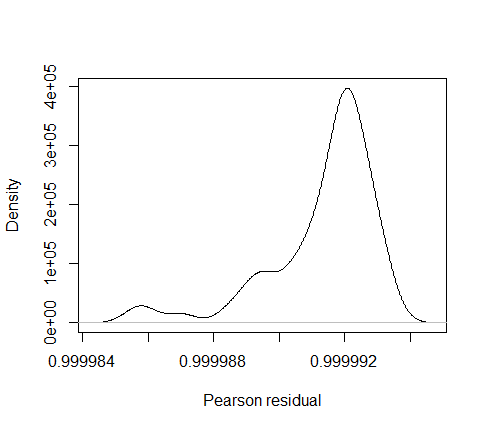
\includegraphics[scale=0.25]{figures/group3_2.png}\label{sublogisGroup3Subgroup2}
      }
      \quad
      \subfigure[Pearson residual of Group3 subgroup3]{
      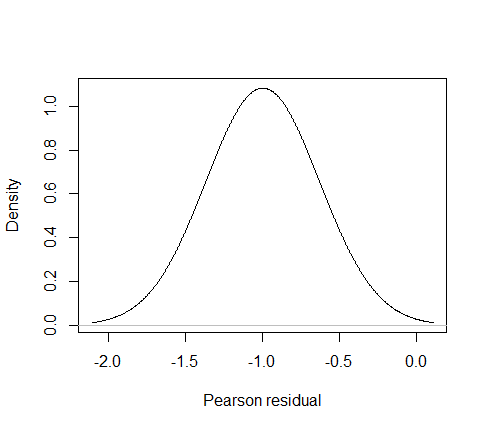
\includegraphics[scale=0.25]{figures/group3_3.png}\label{sublogisGroup3Subgroup3}
      }
      \caption{\small{Kernel density plot of the Pearson residuals of subgroups in Group3 identifed by the LLM model with sublogistic regressions.}}
      \end{figure}

\begin{figure}[htbp]
      \centering
      \subfigure[Pearson residual of Group4 subgroup1]{
      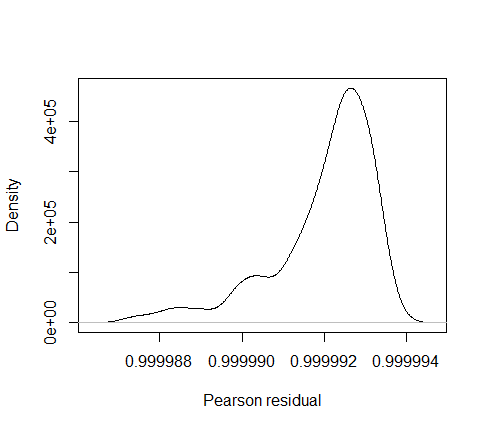
\includegraphics[scale=0.25]{figures/group4_1.png}\label{sublogisGroup4Subgroup1}
      }
      \quad
      \subfigure[Pearson residual of Group4 subgroup2]{
      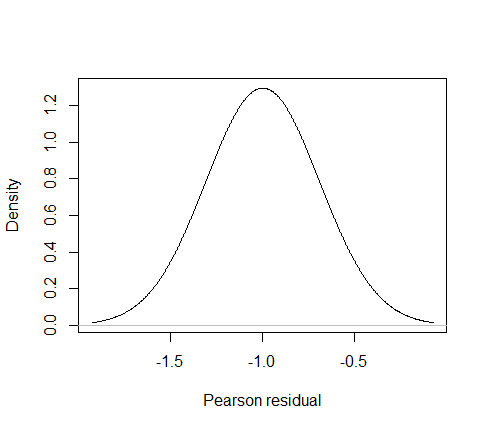
\includegraphics[scale=0.25]{figures/group4_2.png}\label{sublogisGroup4Subgroup2}
      }
      \caption{\small{Kernel density plot of the Pearson residuals of subgroups in Group4 identifed by the LLM model with sublogistic regressions.}}
      \end{figure}
      
\begin{figure}[htbp]
      \centering
      \subfigure[Pearson residual of Group5 subgroup1]{
      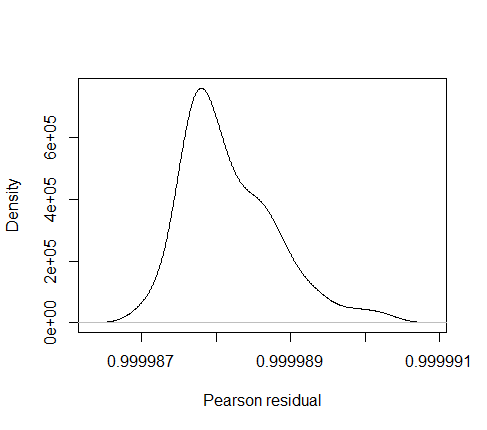
\includegraphics[scale=0.25]{figures/group5_1.png}\label{sublogisGroup5Subgroup1}
      }
      \quad
      \subfigure[Pearson residual of Group5 subgroup2]{
      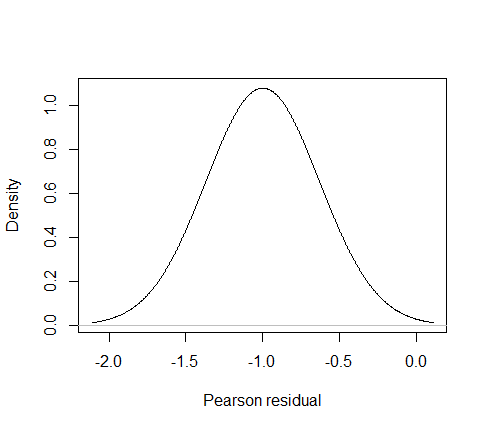
\includegraphics[scale=0.25]{figures/group5_2.png}\label{sublogisGroup5Subgroup2}
      }
      \caption{\small{Kernel density plot of the Pearson residuals of subgroups in Group5 identifed by the LLM model with sublogistic regressions.}}
      \end{figure}
\end{document}                          % The required last line